\documentclass[a4paper,11pt]{article}
\input{/home/tof/Documents/Cozy/latex-include/preambule_lua.tex}
\newcommand{\showprof}{show them}  % comment this line if you don't want to see todo environment
\fancyhead[L]{Portes logiques - partie 2}
\newdate{madate}{10}{09}{2020}
\fancyhead[R]{Première - NSI} %\today
\fancyfoot[L]{~\\Christophe Viroulaud}
\fancyfoot[C]{\textbf{Page \thepage}}
\fancyfoot[R]{\includegraphics[width=2cm,align=t]{/home/tof/Documents/Cozy/latex-include/cc.png}}

\begin{document}
\begin{Form}
\setcounter{section}{2}
\section{Combinaison de transistors}
\begin{commentprof}
\textbf{Activité:} Par groupe de 2: chacun choisit une combinaison et réalise la table de logique. Puis comparer.
\end{commentprof}
\subsection{Porte NAND}
\begin{figure}[!h]
\centering
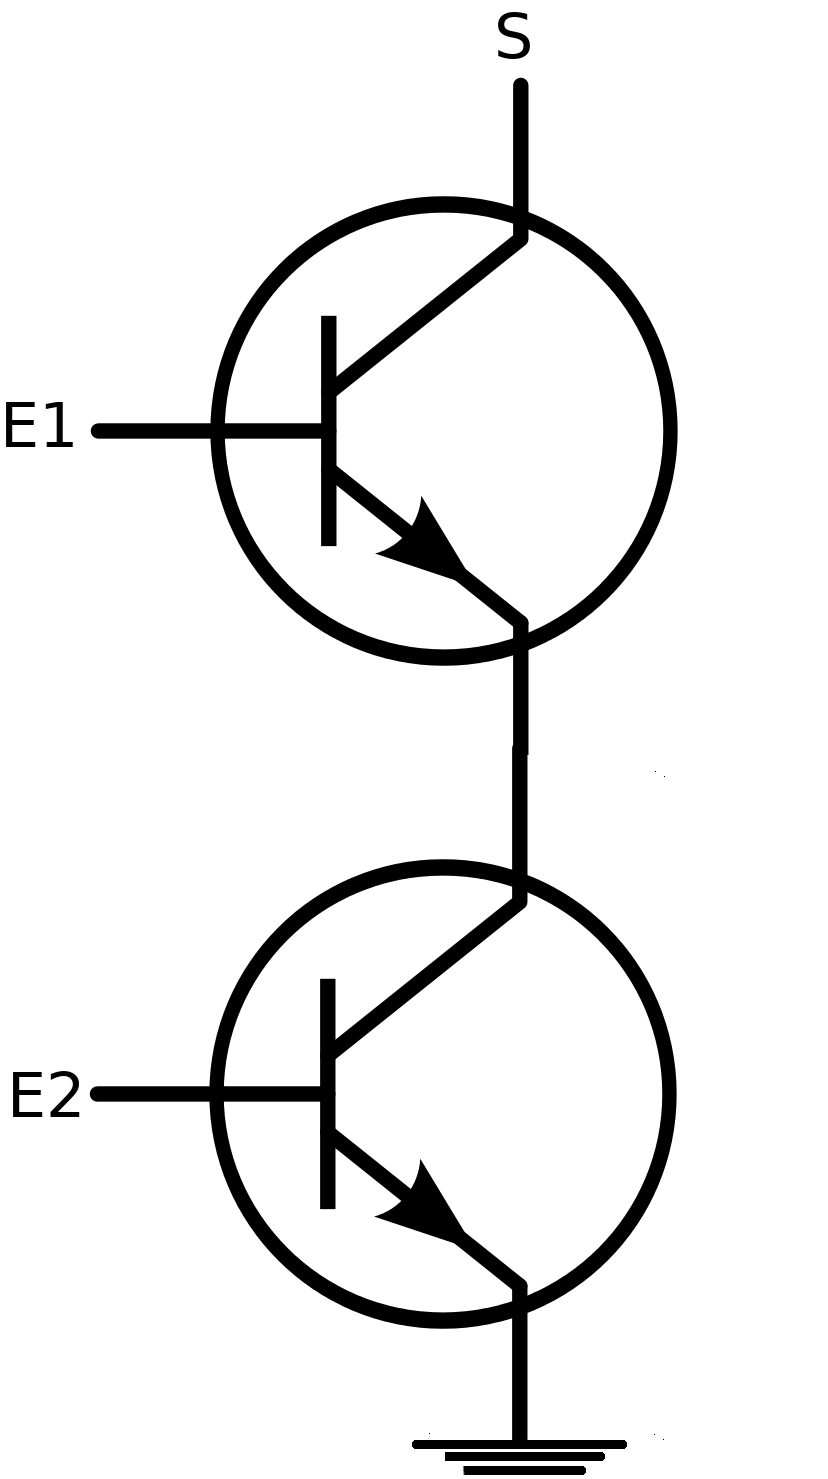
\includegraphics[width=3cm]{ressources/schema-nand.png}
\captionof{figure}{Montage en série}
\label{nand}
\end{figure}
\begin{commentprof}
schéma simplifié; normalement rajoute résistances pour éviter court-circuit
\end{commentprof}
\begin{table}[!h]
\begin{center}
\begin{tabular}{|c|c|c|}
\hline 
E1 & E2 & S \\ 
\hline 
0 & 0 & 1 \\ 
\hline 
0 & 1 & 1\\ 
\hline 
1 & 0 & 1\\
\hline 
1 & 1 & 0\\
\hline 
\end{tabular}
\caption{\label{not}Fonction NAND}
\end{center}
\end{table} 
\begin{center}
\begin{tabular}{*{2}{>{\centering\arraybackslash}m{.4\textwidth}}}
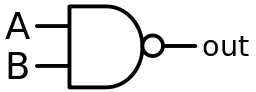
\includegraphics[width=5cm]{ressources/not-and-us.png}
  & 
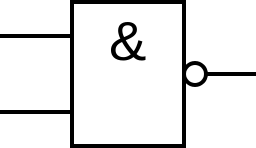
\includegraphics[width=5cm]{ressources/not-and-eu.png}  
   \\
Symbole américain & Symbole européen
\end{tabular}
\end{center}
\subsection{Porte NOR}
\begin{figure}[!h]
\centering
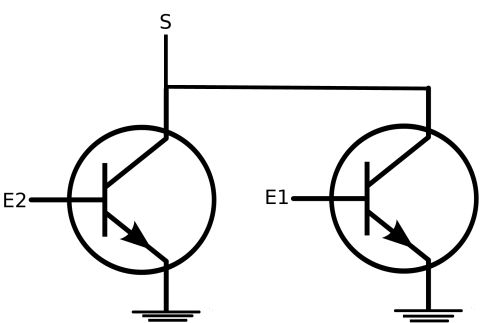
\includegraphics[width=3cm]{ressources/schema-nor.png}
\captionof{figure}{Montage en parallèle}
\label{nand}
\end{figure}
\begin{table}[!h]
\begin{center}
\begin{tabular}{|c|c|c|}
\hline 
E1 & E2 & S \\ 
\hline 
0 & 0 & 1 \\ 
\hline 
0 & 1 & 0\\ 
\hline 
1 & 0 & 0\\
\hline 
1 & 1 & 0\\
\hline 
\end{tabular}
\caption{\label{not}Fonction NOR}
\end{center}
\end{table} 
\begin{center}
\begin{tabular}{*{2}{>{\centering\arraybackslash}m{.4\textwidth}}}
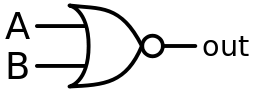
\includegraphics[width=5cm]{ressources/not-or-us.png}
  & 
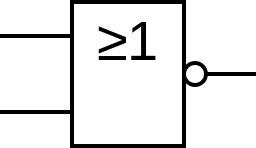
\includegraphics[width=5cm]{ressources/not-or-eu.png}  
   \\
Symbole américain & Symbole européen
\end{tabular}
\end{center}
\section{Combinaison de fonctions logiques}
\begin{commentprof}
à partir de nos briques élémentaires, nous pouvons construire d'autres fonctions.
\end{commentprof}
\subsection{Encore une fonction NOT}
Il est possible de fabriquer une porte NOT en reliant les 2 entrées d'une porte NAND.
\begin{figure}[!h]
\centering
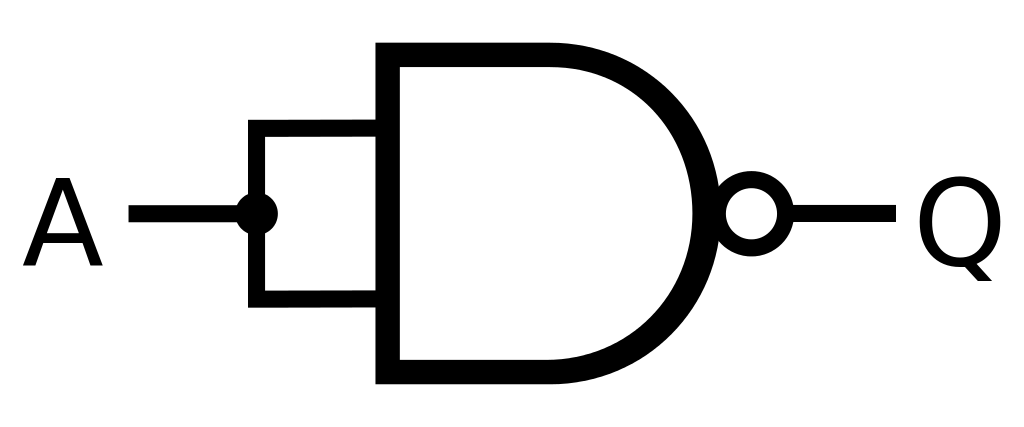
\includegraphics[width=5cm]{ressources/not-from-nand.png}
\captionof{figure}{La porte NOT}
\label{not2}
\end{figure}
\begin{commentprof}
\textbf{Activité:} mêmes instructions que précédemment mais avec combinaison de fonctions logiques.
\end{commentprof}
\subsection{Fonction AND}
\begin{figure}[!h]
\centering
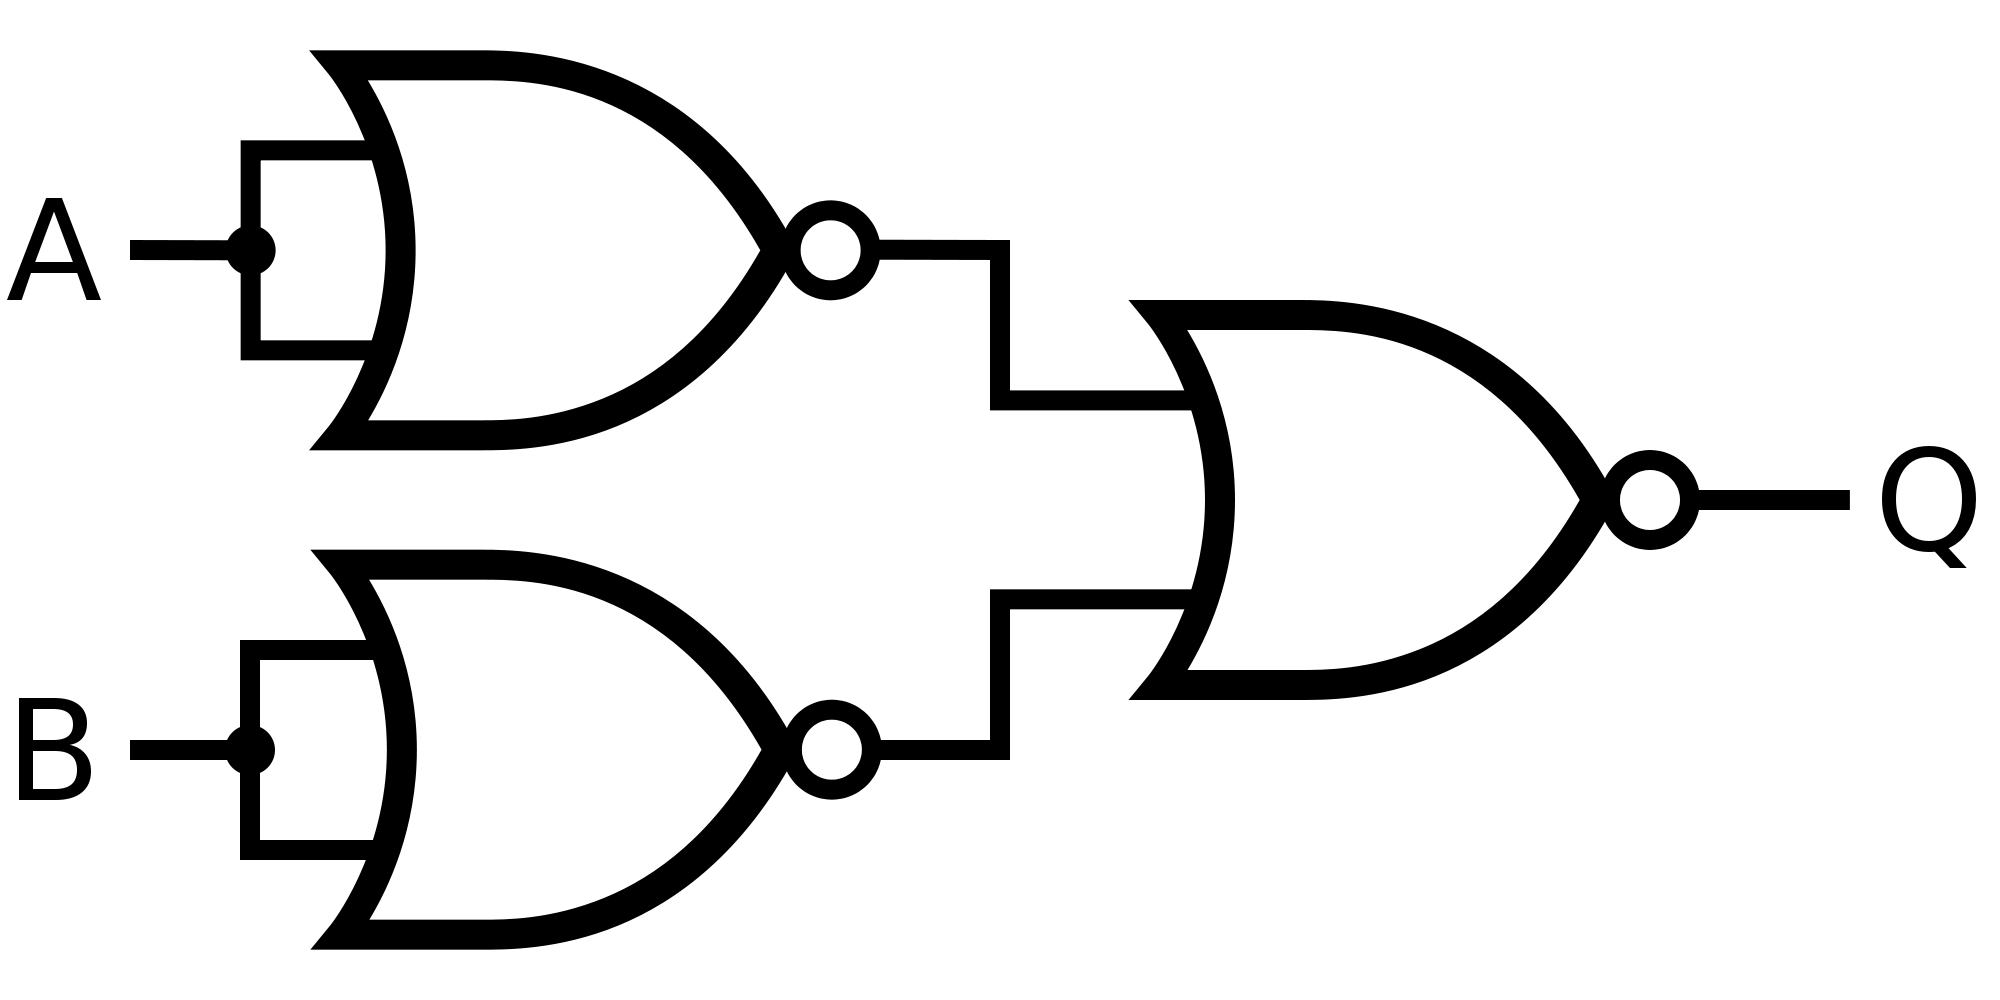
\includegraphics[width=3cm]{ressources/and-from-nor.png}
\captionof{figure}{Porte AND}
\label{and}
\end{figure}
\begin{table}[!h]
\begin{center}
\begin{tabular}{|c|c|c|}
\hline 
A & B & out \\ 
\hline 
0 & 0 & 0 \\ 
\hline 
0 & 1 & 0\\ 
\hline 
1 & 0 & 0\\
\hline 
1 & 1 & 1\\
\hline 
\end{tabular}
\caption{\label{not}Fonction AND}
\end{center}
\end{table} 
\begin{center}
\begin{tabular}{*{2}{>{\centering\arraybackslash}m{.4\textwidth}}}
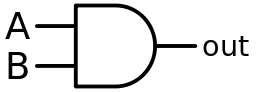
\includegraphics[width=5cm]{ressources/and-us.png}
  & 
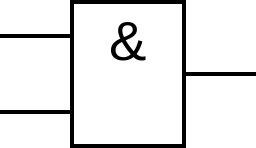
\includegraphics[width=5cm]{ressources/and-eu.png}  
   \\
Symbole américain & Symbole européen
\end{tabular}
\end{center}
\subsection{Fonction OR}
\begin{figure}[!h]
\centering
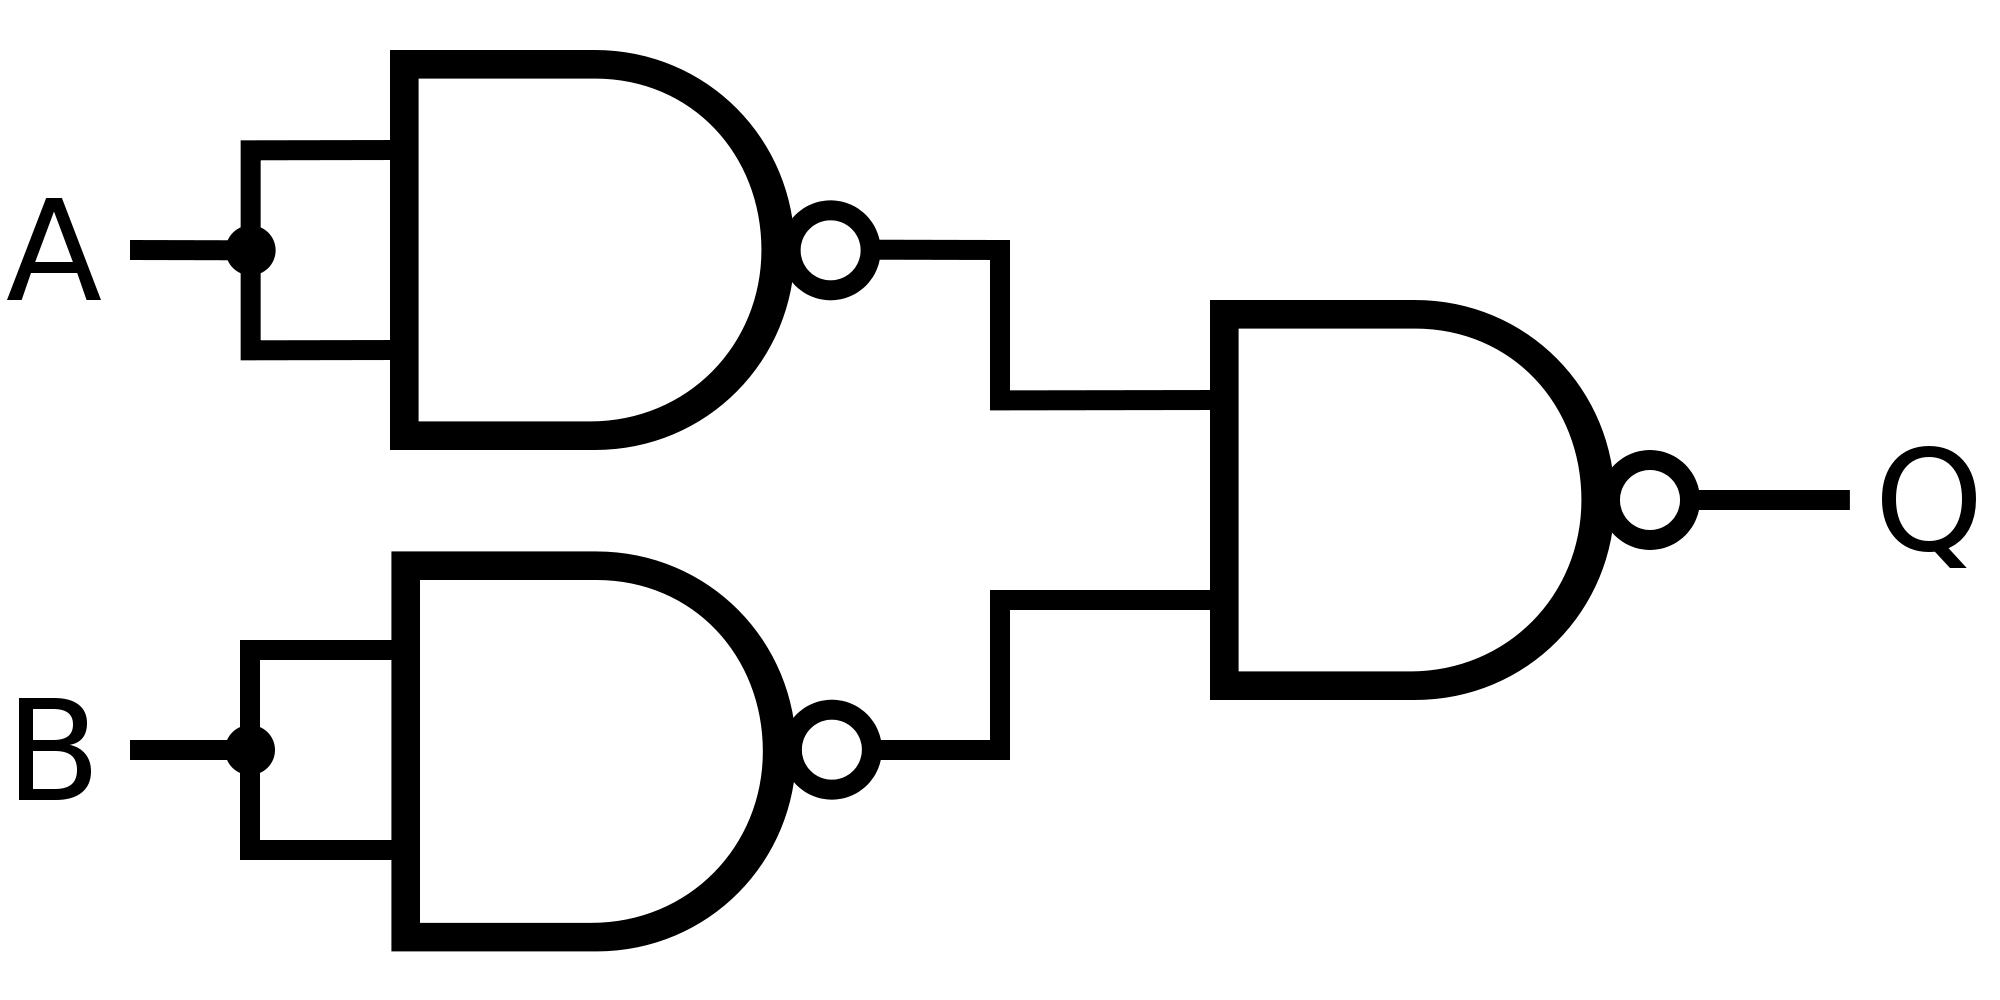
\includegraphics[width=3cm]{ressources/or-from-nand.png}
\captionof{figure}{Porte OR}
\label{nand}
\end{figure}
\begin{table}[!h]
\begin{center}
\begin{tabular}{|c|c|c|}
\hline 
A & B & out \\ 
\hline 
0 & 0 & 0 \\ 
\hline 
0 & 1 & 1\\ 
\hline 
1 & 0 & 1\\
\hline 
1 & 1 & 1\\
\hline 
\end{tabular}
\caption{\label{not}Fonction OR}
\end{center}
\end{table} 
\begin{center}
\begin{tabular}{*{2}{>{\centering\arraybackslash}m{.4\textwidth}}}
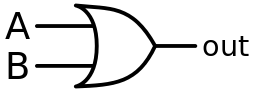
\includegraphics[width=5cm]{ressources/or-us.png}
  & 
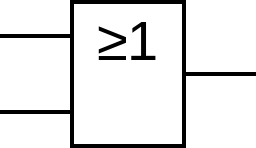
\includegraphics[width=5cm]{ressources/or-eu.png}  
   \\
Symbole américain & Symbole européen
\end{tabular}
\end{center}
\end{Form}
\end{document}